\documentclass{beamer}
\usepackage[italian]{babel} 
 \usetheme{CambridgeUS} 
\usepackage[T1]{fontenc}
\usepackage{amsfonts}
\usepackage{graphicx}
\setbeamertemplate{blocks}[rounded][shadow=true]

\title{Algoritmi per il calcolo parallelo}
\author{...........Author..............}
\date{2021}
 
\subtitle{Equazione dei flussi a superficie libera su griglie strutturate}

\begin{document}
	\frame{\titlepage}
	
	\begin{frame}
		\frametitle{Introduzione}
			Lo scopo di questo progetto consiste nella simulazione di una situazione fluidodinamica: correnti a superficie libera su griglie strutturate.\\
			Con ciò siamo  in grado di osservare non solo la profondità dell’acqua in ogni suo punto, ma anche la conformazione fisica di questa all’interno dell’area di studio.\\
			Per poter così ottimizzare le tempistiche di calcolo, la simulazione potrà essere messa in esecuzione con qualsiasi numero di processori; infatti dimostreremo quanto detto in precedenza, nel momento in cui andremo a guardare i vari tempi di speed-up effettuati con un numero di processori differenti.

	
	\end{frame}

	\begin{frame}
		\frametitle{Condizioni}

		Il nostro dominio di calcolo è: $\Omega$ = $ [ -0.5; 0.5 ] x [ -0.5; 0.5 ]	$, con la condizione iniziale della nostra pressione $\eta$ =  1 + $e^{ -\frac{1}{2* s^{2}} * (x^{2} + y^{2})} $ e \\ \emph{s} = 0.1. c è il tempo con intervallo [0, 0.1]\\
		
		
		Il dominio di calcolo è discretizzato per mezzo di una griglia sfalsata composta da un numero totale: N e M di celle equamente risparmiate con dimensione della maglia($\Delta$x ).
			
		Per questo progetto, abbiamo tralasciato i termini convettivi, cioè :
			\begin{center}
			
			$ \emph{Fu}_{i + \frac{1}{2} j}^{n} = u_{i+\frac{1}{2},j}^{n}	$ e $\emph{Fv}_{i,j + \frac{1}{2}} ^{n}	= u_{i, j +\frac{1}{2},j}^{n}	$
			
			\end{center}	
   	\end{frame}


	\begin{frame}
		
		\frametitle{Condizioni}
		
			\begin{itemize}
				\item Le velocità discrete u($i+\frac{1}{2} ; j $) e v($ i ; j+\frac{1}{2}$) sono definite alle interfacce di celle, mentre la pressione discreta ($\eta$) è data ai baricentri delle celle.\\
				\item $\Delta$t rappresenta il passo temporale.
				\smallskip
				
				\item Ricordiamo brevemente le equazioni di governo per i flussi a superficie libera e introduciamo un metodo numerico adatto per risolverle. Lo schema è basato su una discretizzazione temporale semi-implicit e un’approssimazione spaziale a differenza finita.
				\item Lasciamo che lo spazio fisico sia descritto dal vettore posizione x=(x,y,z), mentre i componenti di velocità in direzione x, y e z sono indicati con u(x, y, z, t), v(x, y, z, t), rispettivamente con t viene indicato  il tempo iniziale.
			\end{itemize}
		
	\end{frame}
	
	
	\begin{frame}
		\frametitle{Condizioni}
			La profondità totale dell'acqua all'interfaccia è calcolata come: 
	
		\begin{center}
			$ H_{i+\frac{1}{2};j}^{n} $ = $  \max { 0, h_{i + \frac{1}{2}; j}^{n} + \eta_{i;j}^{n} ; h_{i+\frac{1}{2}; j}^{n} + \eta_{i+1;j)^{n} } } $
			
			$ H_{i; j+\frac{1}{2}}^{n} $ = $ \max { 0 , h_{i; j+\frac{1}{2}}^{n} + \eta_{i;j}^{n}; h_{i; j+\frac{1}{2}}^{n}+ \eta_{i; j+1)} } $
		\end{center}
	
			
	\end{frame}
	
	\begin{frame}
		\frametitle{Costruzione dell'equazione dei flussi a superficie libera su griglie strutturate }
			Abbiamo un sistema di tre equazioni: due per le velocità del fluido e uno per la pressione, cioè la sua altezza.\\
			Se ipotizziamo di avere un fondo piatto, la nostra H è la pressione del nostro fluido.\\
			Sostanzialmente, la pressione rappresenta l’altezza del fluido in un determinato punto e momento.
			
	\end{frame}

	\begin{frame}
		\frametitle{Condizioni iniziali}
		\begin{itemize}
		\item Le velocità discrete u($i+\frac{1}{2} ; j $) e v($ i ; j+\frac{1}{2}$) sono definite alle interfacce delle celle, mentre la pressione discreta ($\eta$) è data ai baricentri delle celle.\\
		\item $\Delta$t rappresenta il passo temporale.
		\smallskip
		
		\item Ricorderemo brevemente le equazioni di governo per i flussi a superficie libera e introdurremo un metodo numerico adatto per risolverle. Lo schema è basato su una discretizzazione temporale semi-implicit e un'approssimazione spaziale a differenza finita.
		\item Lasciamo che lo spazio fisico sia descritto dal vettore posizione x=(x,y,z), mentre gli componenti di velocità in direzione x, y e z siano indicati con u(x, y, z, t), v(x, y, z, t), rispettivamente con t inizia il tempo.
		\end{itemize}
	\end{frame}


	\begin{frame}
		Come nella modellazione in 1D, affinché la soluzione ($\eta$) possa evolvere nel tempo, istante per istante, possiamo utilizzare una discretizzazione esplicita risolvendo :
		\begin{center}
				
				$ \eta_{i ; j}^{n+1} = \eta_{i ;j} ^{n}  - g*\frac{\Delta t}{\Delta x} *( H_{i+ \frac{1}{2} ; j}^n u_{i+\frac{1}{2};j}^{n+1} - H_{i-\frac{1}{2};j}^{n} u_{i-\frac{1}{2};j}^{n}) $ \\
				$\frac{\Delta t}{\Delta y} *( H_{i; j+ \frac{1}{2}}^{n} v_{i; j+\frac{1}{2}}^{n+1} - H_{i;j-\frac{1}{2}}^{n} v_{i;j-\frac{1}{2}}^{n}) $ 
		\end{center}
		tuttavia questo ci limiterebbe fortemente nella scelta di $\Delta t$, per far si che la condizione di stabilità sia rispettata; è infatti necessario che la velocità del modello numerico adottato sia maggiore della velocità dell'equazione.
	\end{frame}

\begin{frame}
	\frametitle{Sistema lineare}
		Altra soluzione consiste nell'utilizzo di una discretizzazione implicita che ci porta ad un sistema di equazioni risolvibile per sostituzione:
		
		\begin{center}
			$ u_{i + \frac{1}{2} ; j}^{n+1} = Fu_{i + \frac{1}{2}; j} ^{n}  - g*\frac{\Delta t}{\Delta x} *( \eta_{i+1; j} ^{n+1} -\eta_{i; j} ^{n+1}) $
		
		$ v_{i ; j + \frac{1}{2}}^{n+1} = Fv_{i;j  + \frac{1}{2}} ^{n}  - g*\frac{\Delta t}{\Delta y} *( \eta_{i; j+1} ^{n+1} -\eta_{i; j} ^{n+1}) $
		
		$ \eta_{i ; j}^{n+1} = \eta_{i ;j} ^{n}  - g*\frac{\Delta t}{\Delta x} *( H_{i+ \frac{1}{2} ; j}^n u_{i+\frac{1}{2};j}^{n+1} - H_{i-\frac{1}{2};j}^{n} u_{i-\frac{1}{2};j}^{n}) $ \\
		$\frac{\Delta t}{\Delta y} *( H_{i; j+ \frac{1}{2}}^{n} v_{i; j+\frac{1}{2}}^{n+1} - H_{i;j-\frac{1}{2}}^{n} v_{i;j-\frac{1}{2}}^{n}) $ 
		\end{center}
		$\'E$ un sistema pentadiagonale.
\end{frame}

\begin{frame}
	L'equazione che ricaviamo, tramite le varie sostituzioni è:
	
	\medskip
	
	$ \eta_{i;j}^{n} - \frac{\Delta t}{\Delta x}Hx_{i+\frac{1}{2};j}^{n} Fu_{i+\frac{1}{2};j} + \frac{\Delta t^{2}}{\Delta x^{2}}Hx_{i-\frac{1}{2};j}^{n} Fu_{i-\frac{1}{2};j} -\frac{\Delta t^{2}}{\Delta y^{2}}Hy_{i;j+\frac{1}{2}}^{n} Fv_{i;j+\frac{1}{2}}  + \frac{\Delta t^{2}}{\Delta y^{2}}Hy_{i;j-\frac{1}{2}}^{n} Fv_{i;j-\frac{1}{2}} = -g\frac{\Delta t^{2}}{\Delta x^{2}}Hy_{i;j-\frac{1}{2}}^{n} \eta_{i;j-1} -g\frac{\Delta t^{2}}{\Delta x^{2}}Hx_{i;j-\frac{1}{2}}^{n}  \eta_{i-1;j} + (1 + g(\frac{\Delta t^{2}}{\Delta x^{2}}Hx_{i+\frac{1}{2}; j}^{n} +\frac{\Delta t^{2}}{\Delta x^{2}}Hx_{i-\frac{1}{2}; j}^{n} + \frac{\Delta t^{2}}{\Delta y^{2}}Hy_{i;j+\frac{1}{2}}^{n} + \frac{\Delta t^{2}}{\Delta y^{2}}Hy_{i;j-\frac{1}{2}}^{n} ) )\eta_{i;j}^{n+1} - g\frac{\Delta t^{2}}{\Delta x^{2}}Hx_{i+;\frac{1}{2} ; j}^{n}  \eta_{i+1;j}^{n+1} - g\frac{\Delta t^{2}}{\Delta y^{2}}Hy_{i+;\frac{1}{2} ; j}^{n}  \eta_{i;j+1}^{n+1}	$
\end{frame}


\begin{frame}
	\frametitle{Plot dei risultati }
	
	\begin{figure}
		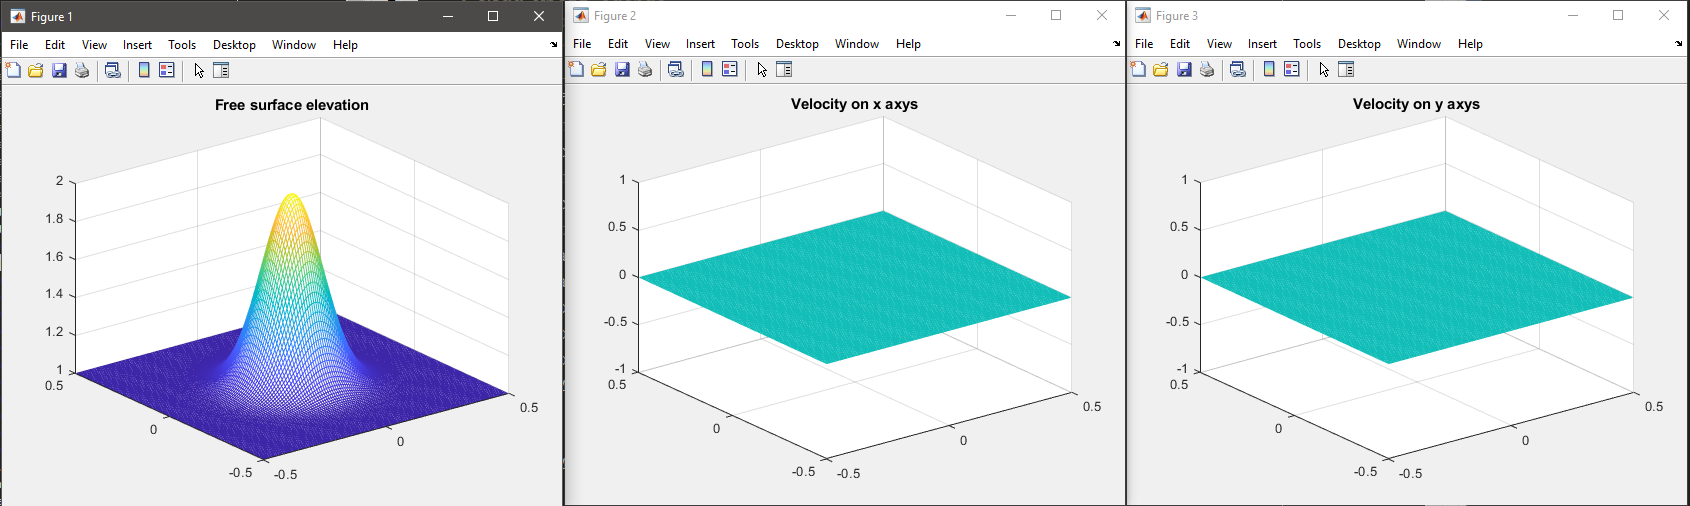
\includegraphics[width=1.0\linewidth]{test_2_cpu_matrice_120_120_0000_0000}
		\caption{Rappresentazione velocità sull'asse x e y}
		\label{fig:Rappresentazione velocità sull'asse x e y}
	\end{figure}
	
\end{frame}


\begin{frame}
	\frametitle{Plot dei risultati }
	\begin{figure}
	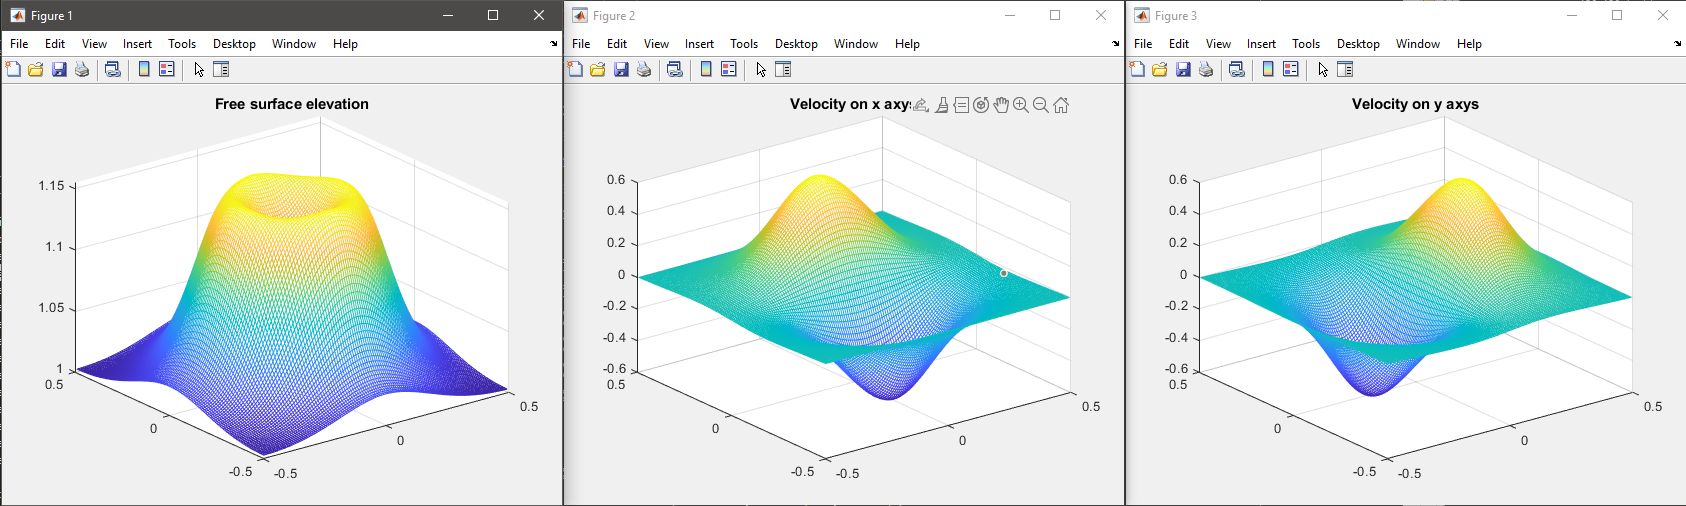
\includegraphics[width=1.0\linewidth]{test_2_cpu_matrice_120_120_0003_0000}
	\caption{Rappresentazione free surface elevation al tempo intermedio}
	\label{fig:Rappresentazione free surface elevation al tempo intermedio}

	\end{figure}
\end{frame}
\begin{frame}
	\frametitle{Plot dei risultati }
	\begin{figure}
	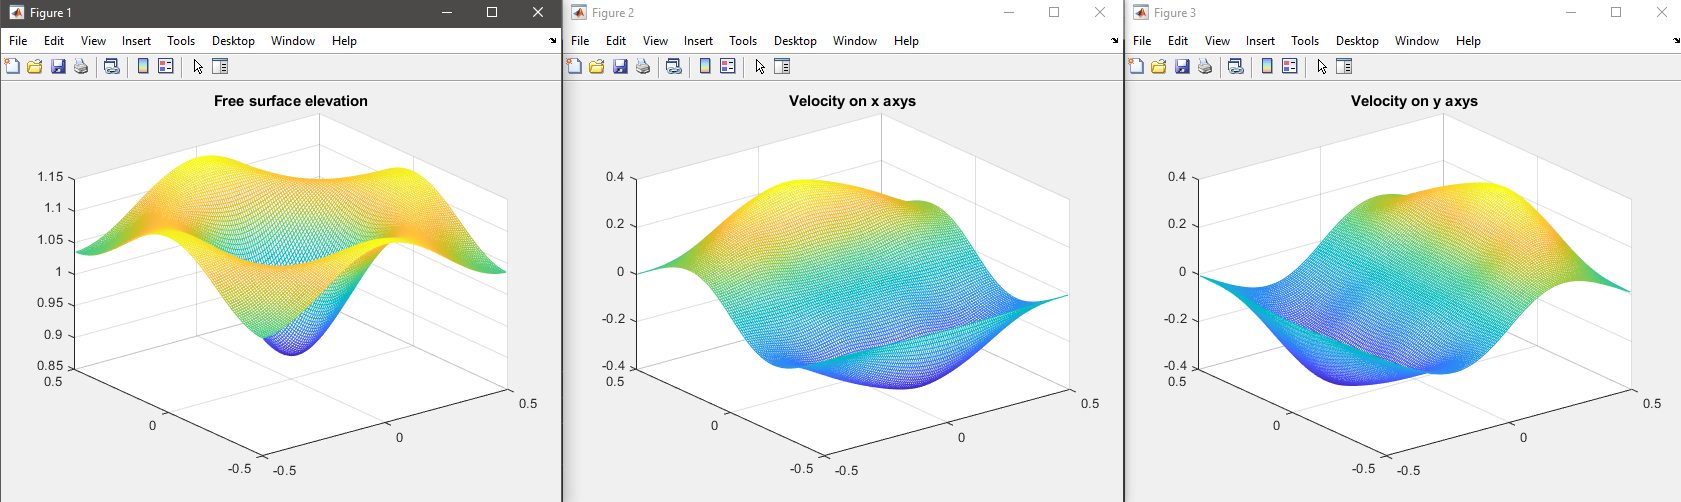
\includegraphics[width=1.0\linewidth]{test_2_cpu_matrice_120_120_0008_0000}
	\caption{Rappresentazione free surface elevation al tempo finale}
	\label{fig:Rappresentazione free surface elevation al tempo finale}
	\end{figure}
\end{frame}


\begin{frame}
	\frametitle{Idea generale}
	
	Definiamo delle matrici dove le \textcolor{blue}{\textbf{I}} vengono lasciate come sono, mentre sulla base di \textcolor{blue}{\textbf{J}} vengono divise. Si ha quindi una divisione orizzontale.\\
	Le matrici vengono definite  da i\textcolor{blue}{\emph{istart -1}} a \textcolor{blue}{\emph{jend +1}}, quindi quello che stiamo facendo è andare a riservarci una colonna in più a sinistra e a destra.\\
	Per prima cosa, ci calcoliamo il valore che ci interessa tra \textcolor{blue}{\emph{istart}} a \textcolor{blue}{\emph{iend}}.
	Dopo aver ottenuto il risultato, passiamo le informazioni alla colonna precedente e successiva in maniera tale che si salvi il risultato.
	Con questo metodo possiamo ottenere i valori corretti e interscambiare il valore sulla riga con la colonna e viceversa.
	Facendo così possiamo ottenere le informazioni da parte degli altri processori e ottenere il risultato finale.
	 
	
\end{frame}
\begin{frame}
	\frametitle{Parallelizzazione}
	Il numero di processori utilizzati per l'esecuzione è dato come parametro di avvio del programma, in maniera tale da suddividere la griglia cartesiana tra gli n processori utilizzati, in modo tale che ciascuno possa operare su una porzione di questa.
	Infatti, abbiamo una distribuzione degli elementi orizzontale, cioè: \textcolor{blue}{nElement = JMAX/ MPI$\%$nCPU}, si è utilizzato solo l'asse y, creando dei rettangoli.\\
	
	Inoltre, definiamo delle matrici con una determinata dimensione, e solo per quelle di cui ho bisogno delle matrici ausiliare, quindi dei buffer. \\
	I buffer sono vettori con lo scopo di contenere le informazioni delle celle vicine.
	
\end{frame}
\begin{frame}
	\frametitle{Parallelizzazione}
	Al momento della produzione di un file di output, tutte le porzioni aggiornate devono essere riunite all'interno del processore.
	Per ottenere tale risultato ci serviamo della subroutine MPI$\_$GATHER che svolge proprio questo compito. \\
	
	Affinché possa avvenire l'unificazione dei dati all'interno di una matrice, andiamo a ciclare sulla MPI$\_$ALLGATHER con i buffer.
\end{frame}

\begin{frame}
	\frametitle{Risultati}
	Possiamo vedere i vari risultati che si ottengono con il metodo utilizzato per la parallelizzazione sulla computazione, è necessario effettuare la simulazione con una griglia il più fitta possibile, in modo da rendere veramente oneroso il carico di lavoro.\\
	
	Ad esempio, utilizzando una griglia 120 x 120 si ottengono i seguenti risultati:
	
	\smallskip
	\begin{center}
		\begin{tabular}{|l|l|l|r|}
			\hline
			N. di processori & tempo1 & tempo2 & tempo3\\
			\hline
			1 & 6.71857500 &  & a\\
			\hline
			2 & 5.1161794 & & a\\
			\hline
		
		\end{tabular}
	
	\end{center}
	
\end{frame}



\begin{frame}
	\frametitle{Speedup}
	Formula speedup:
	
	\begin{center}
		$ S(p) = \dfrac{T_{(p=1)}}{T(p)} $
	\end{center}
		dove T(1) è il tempo medio di calcolo con \textcolor{blue}{1 solo processore} (seriale), mentre T(p) è il tempo medio ottenuto con \textcolor{blue}{p} processori
	
\end{frame}

\begin{frame}
	\frametitle{Efficienza}
	Formula efficienza:
	
	\begin{center}
		$ E(p) = \dfrac{S(p)}{p} $
	\end{center}
quindi sarebbe il rapporto tra speedup e numero di processori.

	
\end{frame}

\begin{frame}
	\frametitle{Funzione di Kuck}
	Formula funzione di Kuck:
	
	\begin{center}
		$ K(p) = S(p)* E(p) $
	\end{center}
	il numero di processori è il massimo di K(p) ottenendo il miglior compromesso tra speedup ed efficienza.  
	
	
\end{frame}

\end{document}